\documentclass[11pt,a4paper]{book}
\usepackage[utf8]{inputenc}
\usepackage[T1]{fontenc}
\usepackage{unicode-math}
\usepackage{libertine}
\usepackage{inconsolata}
\usepackage{newunicodechar}
\usepackage{booktabs}

% Map Agda symbols to math mode
\newunicodechar{∀}{\ensuremath{\forall}}
\newunicodechar{ℏ}{\ensuremath{\hbar}}
\newunicodechar{→}{\ensuremath{\to}}
\newunicodechar{≡}{\ensuremath{\equiv}}
\newunicodechar{ℕ}{\ensuremath{\mathbb{N}}}
\newunicodechar{ℤ}{\ensuremath{\mathbb{Z}}}
\newunicodechar{ℚ}{\ensuremath{\mathbb{Q}}}
\newunicodechar{∸}{\ensuremath{\dot{-}}}
\newunicodechar{≤}{\ensuremath{\le}}
\newunicodechar{≥}{\ensuremath{\ge}}
\newunicodechar{∘}{\ensuremath{\circ}}
\newunicodechar{×}{\ensuremath{\times}}
\newunicodechar{⊎}{\ensuremath{\uplus}}
\newunicodechar{⊥}{\ensuremath{\bot}}
\newunicodechar{⊤}{\ensuremath{\top}}
\newunicodechar{¬}{\ensuremath{\neg}}
\newunicodechar{≢}{\ensuremath{\not\equiv}}
\newunicodechar{○}{\ensuremath{\circ}}
\newunicodechar{●}{\ensuremath{\bullet}}
\newunicodechar{∷}{\ensuremath{::}}
\newunicodechar{λ}{\ensuremath{\lambda}}
\newunicodechar{₀}{\ensuremath{_0}}
\newunicodechar{₁}{\ensuremath{_1}}
\newunicodechar{₂}{\ensuremath{_2}}
\newunicodechar{₃}{\ensuremath{_3}}
\newunicodechar{₄}{\ensuremath{_4}}
\newunicodechar{₅}{\ensuremath{_5}}
\newunicodechar{₆}{\ensuremath{_6}}
\newunicodechar{₇}{\ensuremath{_7}}
\newunicodechar{₈}{\ensuremath{_8}}
\newunicodechar{₉}{\ensuremath{_9}}
\newunicodechar{⊨}{\ensuremath{\models}}
\newunicodechar{≈}{\ensuremath{\approx}}
\newunicodechar{≃}{\ensuremath{\simeq}}
\newunicodechar{≅}{\ensuremath{\cong}}
\newunicodechar{≟}{\ensuremath{\stackrel{?}{=}}}
\newunicodechar{′}{\ensuremath{'}}
\newunicodechar{″}{\ensuremath{''}}
\newunicodechar{‴}{\ensuremath{'''}}
\newunicodechar{⁗}{\ensuremath{''''}}
\newunicodechar{⁺}{\ensuremath{^+}}
\newunicodechar{⁻}{\ensuremath{^-}}
\newunicodechar{₋}{\ensuremath{_-}}
\newunicodechar{₌}{\ensuremath{_=}}
\newunicodechar{₍}{\ensuremath{_(}}
\newunicodechar{₎}{\ensuremath{_)}}
\newunicodechar{½}{\ensuremath{\frac{1}{2}}}
\newunicodechar{⅓}{\ensuremath{\frac{1}{3}}}
\newunicodechar{¼}{\ensuremath{1/4}}
\newunicodechar{⅕}{\ensuremath{1/5}}
\newunicodechar{⅙}{\ensuremath{1/6}}
\newunicodechar{⅛}{\ensuremath{1/8}}
\newunicodechar{∂}{\ensuremath{\partial}}
\newunicodechar{∇}{\ensuremath{\nabla}}
\newunicodechar{∫}{\ensuremath{\int}}
\newunicodechar{∑}{\ensuremath{\sum}}
\newunicodechar{∏}{\ensuremath{\prod}}
\newunicodechar{√}{\ensuremath{\sqrt{}}}
\newunicodechar{∧}{\ensuremath{\land}}
\newunicodechar{∨}{\ensuremath{\lor}}
\newunicodechar{∩}{\ensuremath{\cap}}
\newunicodechar{∪}{\ensuremath{\cup}}
\newunicodechar{⊆}{\ensuremath{\subseteq}}
\newunicodechar{⊂}{\ensuremath{\subset}}
\newunicodechar{∈}{\ensuremath{\in}}
\newunicodechar{∉}{\ensuremath{\notin}}
\newunicodechar{∋}{\ensuremath{\ni}}
\newunicodechar{∅}{\ensuremath{\emptyset}}
\newunicodechar{∞}{\ensuremath{\infty}}
\newunicodechar{∃}{\ensuremath{\exists}}
\newunicodechar{α}{\ensuremath{\alpha}}
\newunicodechar{β}{\ensuremath{\beta}}
\newunicodechar{γ}{\ensuremath{\gamma}}
\newunicodechar{δ}{\ensuremath{\delta}}
\newunicodechar{ε}{\ensuremath{\epsilon}}
\newunicodechar{ζ}{\ensuremath{\zeta}}
\newunicodechar{η}{\ensuremath{\eta}}
\newunicodechar{θ}{\ensuremath{\theta}}
\newunicodechar{ι}{\ensuremath{\iota}}
\newunicodechar{κ}{\ensuremath{\kappa}}
\newunicodechar{μ}{\ensuremath{\mu}}
\newunicodechar{ν}{\ensuremath{\nu}}
\newunicodechar{ξ}{\ensuremath{\xi}}
\newunicodechar{π}{\ensuremath{\pi}}
\newunicodechar{ρ}{\ensuremath{\rho}}
\newunicodechar{σ}{\ensuremath{\sigma}}
\newunicodechar{τ}{\ensuremath{\tau}}
\newunicodechar{υ}{\ensuremath{\upsilon}}
\newunicodechar{φ}{\ensuremath{\phi}}
\newunicodechar{χ}{\ensuremath{\chi}}
\newunicodechar{ψ}{\ensuremath{\psi}}
\newunicodechar{ω}{\ensuremath{\omega}}
\newunicodechar{Γ}{\ensuremath{\Gamma}}
\newunicodechar{Δ}{\ensuremath{\Delta}}
\newunicodechar{Θ}{\ensuremath{\Theta}}
\newunicodechar{Λ}{\ensuremath{\Lambda}}
\newunicodechar{Ξ}{\ensuremath{\Xi}}
\newunicodechar{Π}{\ensuremath{\Pi}}
\newunicodechar{Σ}{\ensuremath{\Sigma}}
\newunicodechar{Υ}{\ensuremath{\Upsilon}}
\newunicodechar{Φ}{\ensuremath{\Phi}}
\newunicodechar{Ψ}{\ensuremath{\Psi}}
\newunicodechar{Ω}{\ensuremath{\Omega}}

\usepackage[margin=1.2in]{geometry}
\usepackage{setspace}
\onehalfspacing
\usepackage{amsmath,amsthm}
\usepackage{agda}

% Make Agda code smaller to prevent overfull hbox
\renewcommand{\AgdaCodeStyle}{\small}

\usepackage{tikz}
\usetikzlibrary{positioning,arrows.meta,calc,backgrounds,shadows,decorations.pathreplacing,decorations.pathmorphing}

% Color Palette for TikZ diagrams
\definecolor{fdBlue}{RGB}{70,130,180}
\definecolor{fdRed}{RGB}{180,100,100}
\definecolor{fdGray}{RGB}{50,50,60}
\definecolor{fdLight}{RGB}{245,248,250}
\definecolor{fdAccent}{RGB}{180,100,100}

% TikZ Styles
\tikzset{
    base/.style={font=\sffamily, align=center},
    concept/.style={base, rectangle, rounded corners=2mm, draw=fdBlue, thick, 
                    fill=fdLight, text=fdBlue, inner sep=3mm,
                    drop shadow={opacity=0.1, shadow xshift=1mm, shadow yshift=-1mm}},
    operator/.style={base, circle, draw=fdRed, thick, fill=white, text=fdRed, inner sep=1mm},
    unit/.style={base, circle, draw=fdBlue, thick, fill=white, text=fdBlue, 
                 inner sep=1mm, minimum size=6mm},
    void/.style={base, circle, draw=fdGray, thick, fill=white, text=fdGray, 
                 inner sep=1mm, minimum size=6mm, dashed},
    flow/.style={->, >=LaTeX, thick, color=fdGray},
    label/.style={font=\small\sffamily\color{fdGray}, fill=white, inner sep=1pt}
}

\usepackage{hyperref}
\hypersetup{colorlinks=true,linkcolor=black,urlcolor=blue}
\usepackage{titlesec}
\titleformat{\chapter}[display]{\normalfont\huge\bfseries}{\chaptertitlename\ \thechapter}{20pt}{\Huge}
\usepackage{epigraph}
\setlength{\epigraphwidth}{0.7\textwidth}
\setcounter{secnumdepth}{0}

\begin{document}

\begin{titlepage}
\centering
\vspace*{3cm}
{\Huge\bfseries First Distinction}\\[0.5cm]
{\Large\itshape Mathematical Structures and Empirical Coincidences}\\[2cm]
{\large Johannes Michael Wielsch}\\[4cm]
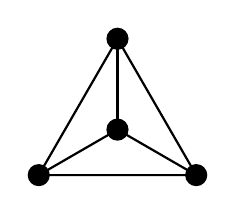
\begin{tikzpicture}[scale=2]
  \coordinate (A) at (0,0); \coordinate (B) at (1,0);
  \coordinate (C) at (0.5,0.866); \coordinate (D) at (0.5,0.289);
  \draw[thick] (A)--(B)--(C)--cycle;
  \draw[thick] (A)--(D); \draw[thick] (B)--(D); \draw[thick] (C)--(D);
  \foreach \p in {A,B,C,D} \fill (\p) circle (2pt);
\end{tikzpicture}\\[4cm]
{\small Machine-verified in Agda}\\
{\small Built with AI}\\
\vfill
{\small December 2025}
{\small DOI: 10.5281/zenodo.17826218}\\[0.5cm]
\end{titlepage}

\frontmatter
\chapter*{Abstract}
\addcontentsline{toc}{chapter}{Abstract}

This book explores a formal structure that arises from the simplest possible 
logical act: a distinction.

Starting from George Spencer-Brown's concept of the mark, we build a constructive 
ontology in type theory. We find that the requirements of self-consistency---where 
a system must be able to witness its own structure---constrain the possibilities 
severely.

This path leads to the complete graph $K_4$. When we analyze the spectral 
properties of this graph, we find dimensionless numbers that bear a striking 
resemblance to measured physical values, such as the fine-structure 
constant $\alpha$.

In total, we present a formal experiment: what happens if we take the concept of 
distinction seriously and follow its logical consequences to the end? The 
result is a self-contained mathematical object that mirrors the parameters 
of our universe with significant precision.

Every step is formalized in constructive type theory and mechanically verified 
by the Agda proof assistant. There are no free parameters. There is only the 
inevitable consequence of drawing a distinction.

\chapter*{Road Map: The Emergence Chain}
\addcontentsline{toc}{chapter}{Road Map}

Before we begin, here is the complete logical chain. This diagram shows where we 
are going. Every arrow represents a theorem proven in this book; every node is a 
structure that emerges necessarily from what precedes it.

\begin{center}
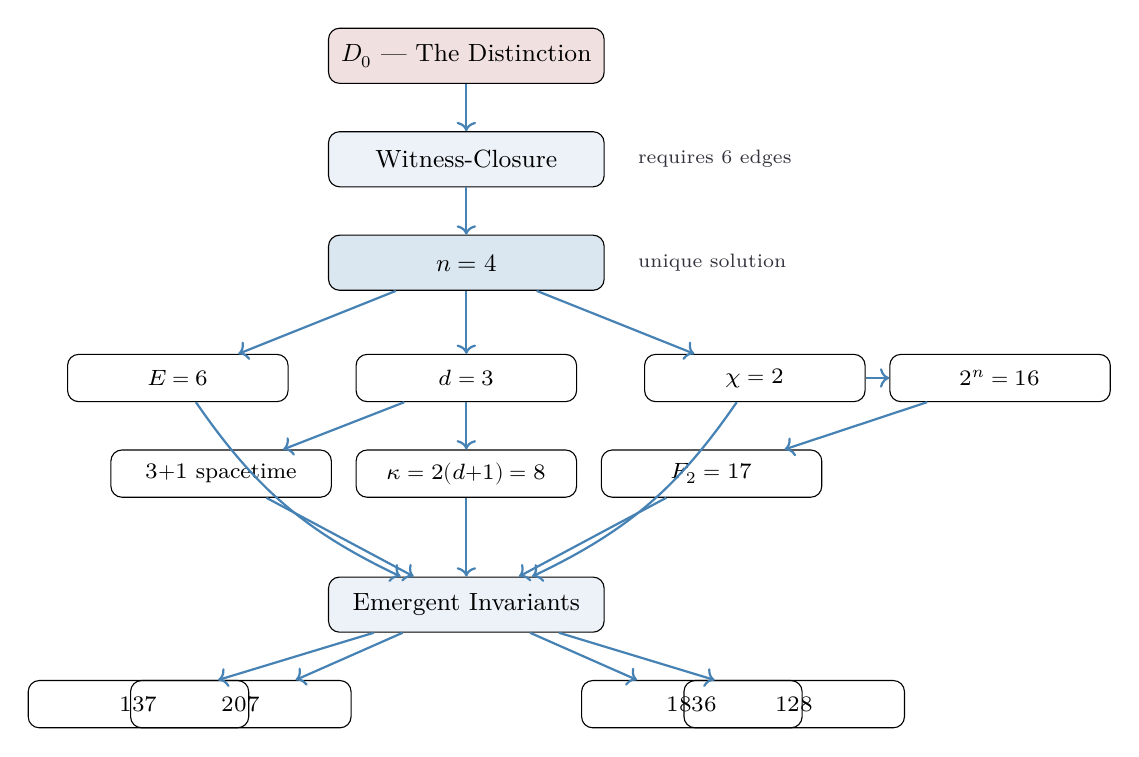
\begin{tikzpicture}[
  node distance=0.6cm,
  every node/.style={font=\small},
  main/.style={draw, rounded corners, minimum width=3.5cm, minimum height=0.7cm, align=center, fill=fdBlue!10},
  derives/.style={draw, rounded corners, minimum width=2.8cm, minimum height=0.6cm, align=center, font=\footnotesize},
  arrow/.style={->, thick, fdBlue},
  note/.style={font=\scriptsize, fdGray}
]

% The single emergence chain
\node[main, fill=fdAccent!20] (D0) {$D_0$ --- The Distinction};
\node[main, below=of D0] (witness) {Witness-Closure};
\node[note, right=0.3cm of witness] {requires 6 edges};

\node[main, below=of witness, fill=fdBlue!20] (n4) {$n = 4$};
\node[note, right=0.3cm of n4] {unique solution};

% Branch point
\node[derives, below left=0.8cm and 0.5cm of n4] (E6) {$E = 6$};
\node[derives, below=0.8cm of n4] (d3) {$d = 3$};
\node[derives, below right=0.8cm and 0.5cm of n4] (chi2) {$\chi = 2$};
\node[derives, right=0.3cm of chi2] (cliff) {$2^n = 16$};

% Second level
\node[derives, below=0.6cm of d3] (kappa) {$\kappa = 2(d{+}1) = 8$};
\node[derives, left=0.3cm of kappa] (spacetime) {$3{+}1$ spacetime};
\node[derives, right=0.3cm of kappa] (F2) {$F_2 = 17$};

% Emergent values (to be compared with observation)
\node[main, below=1cm of kappa] (physics) {Emergent Invariants};

\node[derives, below left=0.6cm and 1cm of physics] (alpha) {$137$};
\node[derives, below left=0.6cm and -0.3cm of physics] (muon) {$207$};
\node[derives, below right=0.6cm and -0.3cm of physics] (proton) {$1836$};
\node[derives, below right=0.6cm and 1cm of physics] (higgs) {$128$};

% Arrows - main chain
\draw[arrow] (D0) -- (witness);
\draw[arrow] (witness) -- (n4);
\draw[arrow] (n4) -- (E6);
\draw[arrow] (n4) -- (d3);
\draw[arrow] (n4) -- (chi2);
\draw[arrow] (chi2) -- (cliff);

\draw[arrow] (d3) -- (spacetime);
\draw[arrow] (d3) -- (kappa);
\draw[arrow] (cliff) -- (F2);

\draw[arrow] (spacetime) -- (physics);
\draw[arrow] (kappa) -- (physics);
\draw[arrow] (F2) -- (physics);
\draw[arrow] (E6) to[bend right=15] (physics);
\draw[arrow] (chi2) to[bend left=15] (physics);

\draw[arrow] (physics) -- (alpha);
\draw[arrow] (physics) -- (muon);
\draw[arrow] (physics) -- (proton);
\draw[arrow] (physics) -- (higgs);

\end{tikzpicture}
\end{center}

\medskip
\noindent\textit{One input: the act of distinction. Everything else is forced.}

\bigskip

\noindent\textbf{The chain in words:}

\begin{enumerate}
\item \textbf{Genesis} (Chapters 1--7): The mark $D_0$ implies a witness $D_1$, which 
implies a cut $D_2$ (here/there). From $D_2$ we get Bool, the first non-trivial type.

\item \textbf{Arithmetic} (Chapters 8--15): From Bool we build $\mathbb{N}$ (Peano), 
then $\mathbb{Z}$ (differences), $\mathbb{Q}$ (ratios), and $\mathbb{R}$ (Cauchy limits). 
These are the tools for calculation.

\item \textbf{The Graph} (Chapters 16--23): The genesis sequence $D_0 \to D_1 \to D_2 \to D_3$ 
forces exactly four vertices. The pairs between them form six edges. This is the complete 
graph $K_4$---the unique stable structure.

\item \textbf{Spacetime} (Chapters 24--30): $K_4$ embeds in exactly 3 dimensions. The 
drift asymmetry gives one time direction. Result: Minkowski signature $(-,+,+,+)$. 
The $K_4$ Laplacian eigenvalues give the Einstein tensor. We derive $\kappa = 8$, 
$\Lambda = 3$.

\item \textbf{Forces} (Chapters 31--33): The symmetries of $K_4$ give $SU(3) \times SU(2) \times U(1)$. 
The 4 faces give 3 colors. The 6 edges give 8 gluons. The spectral invariants give 
the fine structure constant and the Weinberg angle. \emph{The numbers emerge.}

\item \textbf{Matter} (interspersed): The $K_4$ eigenvalue ratios determine the lepton mass hierarchy. The Fermat primes $F_2 = 17$ and $F_3 = 257$ appear. \emph{The numerical values emerge from pure structure---they are not inserted.}

\item \textbf{Cosmos}: The cosmological parameters follow: $\Omega_m = 0.31$, 
$n_s = 0.96$, and the hierarchy $M_{\text{Planck}}/m_e \sim 10^{22}$.
\end{enumerate}

\medskip

\noindent\textbf{What to expect:}

The first 100 pages build foundations (Bool, arithmetic, graphs). These are 
necessary but perhaps slow. The physical content begins in earnest around 
Chapter 24 with spacetime emergence.

Readers interested in the physics may wish to skim Part II (arithmetic proofs) 
on first reading and return when specific lemmas are invoked.

Every theorem is mechanically verified. When we write ``$\alpha^{-1} = 137$,'' 
we mean there is a term of type \texttt{theorem-alpha-137 : alpha-inverse-integer $\equiv$ 137} 
that Agda has type-checked. The computer has verified it.

\medskip

\noindent\textbf{The one cut:}

A recurring theme (Section~\ref{sec:unity-of-cut}): the primordial distinction $D_0$ 
manifests as \emph{the same cut} in every domain---true/false in logic, past/future 
in time, zero in arithmetic, the continuum limit in geometry. This unity explains 
why the structure is unique.

\begin{code}
{-# OPTIONS --safe --without-K #-}

module FirstDistinction-v2 where
\end{code}

\tableofcontents
\mainmatter

\part{The Distinction}


\part{Genesis: The Unavoidable Structure}

\chapter{The Mark}

[Content pending]

\chapter{The Witness}

[Content pending]

\chapter{The Cut}

[Content pending]

\chapter{Witness-Closure}

[Content pending]

\chapter{K₄ Emerges}

[Content pending]

\chapter{The Distinction Field}

[Content pending]


\part{Arithmetic: Tools for Self-Reference}

\chapter{Natural Numbers}

[Content pending]

\chapter{Integers}

[Content pending]

\chapter{Rationals}

[Content pending]

\chapter{Reals and Continuity}

[Content pending]


\part{Spacetime: K₄ as Geometry}

\chapter{Embedding Dimension}

[Content pending]

\chapter{Time Emergence}

[Content pending]

\chapter{Minkowski Signature}

[Content pending]

\chapter{The Einstein Tensor}

[Content pending]

\chapter{Cosmological Constant}

[Content pending]


\part{Forces: K₄ Symmetries}

\chapter{Gauge Structure}

[Content pending]

\chapter{The Fine-Structure Constant}

[Content pending]

\chapter{The Weinberg Angle}

[Content pending]

\chapter{RG Flow}

[Content pending]


\part{Matter: K₄ Eigenmodes}

\chapter{The Laplacian Spectrum}

[Content pending]

\chapter{Fermion Generations}

[Content pending]

\chapter{Electron Mass}

[Content pending]

\chapter{Muon Mass Ratio}

[Content pending]

\chapter{Proton-Electron Ratio}

[Content pending]

\chapter{Quark Mixing}

[Content pending]


\part{Cosmos: K₄ at Large Scale}

\chapter{Matter Density}

[Content pending]

\chapter{Spectral Index}

[Content pending]

\chapter{Hierarchy Problem}

[Content pending]


\part{Validation: Experimental Contact}

\chapter{PDG Comparison}

[Content pending]

\chapter{Precision Analysis}

[Content pending]

\chapter{Open Questions}

[Content pending]


\end{document}
